\documentclass[a4paper,12pt]{article}
\usepackage[polish]{babel}
\usepackage[T1]{fontenc}
\usepackage[utf8]{inputenc}
\usepackage{listings}
\usepackage{graphicx}
\usepackage{hyperref}
\usepackage{amsmath}
\usepackage{geometry}
\geometry{
    a4paper,
    left=25mm,
    right=25mm,
    top=20mm,
    bottom=25mm
}

\title{\textbf{Dokumentacja systemu \texttt{VecEdit}}}
\author{Zespół projektowy: \\
\small Adam Rogowski, Szymon Sawoń, Bartosz Siemaszkiewicz}
\date{\today}

\begin{document}

\maketitle
\tableofcontents

\section{Wstęp}

\texttt{VecEdit} to aplikacja (napisana w~\textbf{C++20}) służąca do edycji prostych
grafik wektorowych. Umożliwia rysowanie, modyfikowanie, grupowanie oraz klonowanie
obiektów graficznych (takich jak prostokąty, okręgi czy wielokąty). 
Program korzysta z biblioteki \textbf{raylib} (w wersji 5.5) do wyświetlania okna, 
rysowania figur na ekranie oraz pobierania zdarzeń wejściowych od użytkownika 
(klawiatura, mysz). Do tworzenia interfejsu graficznego w trybie \emph{immediate mode}
używana jest biblioteka \textbf{RayGui}.  

Aplikacja pozwala na:
\begin{itemize}
    \item rysowanie i edycję kształtów (w tym zmianę koloru, obrysu, przezroczystości),
    \item przesuwanie i skalowanie figur,
    \item grupowanie obiektów (\texttt{FigureGroup}),
    \item cofanie (\texttt{undo}) i ponawianie (\texttt{redo}) operacji dzięki wzorcowi \emph{Command},
    \item zapisywanie projektów do plików wektorowych (\texttt{SVG}) i \emph{bitmapowych} (\texttt{PNG}),
    \item otwieranie, zamykanie i przełączanie się między wieloma zakładkami dokumentów.
\end{itemize}

\section{Wzorce projektowe i ich zastosowanie}

Poniżej przedstawiono zastosowane wewnątrz aplikacji wzorce projektowe,
z uwzględnieniem istotnych elementów w~kodzie oraz komentarzy dotyczących
możliwych zmian (tzw. \emph{wektora zmian}).

\subsection{Kompozyt (\emph{Composite})}
\begin{itemize}
    \item \textbf{Cel:} Umożliwienie traktowania pojedynczych obiektów
    (figury) i grup obiektów (grupy figur) w sposób jednolity, dzięki interfejsowi
    \texttt{Figure}. 
    \item \textbf{Struktura:} 
    \begin{itemize}
      \item \texttt{Figure} -- interfejs \emph{komponentu}. Posiada m.in. metody typu 
      \texttt{accept(visitor)}, które w~implementacjach \emph{Composite} przekazują
      wywołanie wszystkim dzieciom.
      \item \texttt{FigureGroup} -- \emph{kompozyt}, zawiera wektor \texttt{children}
      oraz metody \texttt{addChild(...)} itp.
      \item \texttt{RectFigure}, \texttt{CircleFigure}, \texttt{PolyFigure} -- 
      \emph{konkretne komponenty (liście)}, nie posiadają dzieci.
    \end{itemize}
    \item \textbf{Użycie:} 
    \begin{itemize}
      \item W edytorze (\texttt{Editor}) przy \texttt{groupFigures()} i \texttt{ungroupFigures()}
      łączymy/rozbijamy figury w drzewiastą strukturę.
      \item \texttt{accept(visitor)} w \texttt{FigureGroup} wywołuje
      \texttt{accept} u wszystkich dzieci, co integruje się z~\emph{Visitor}.
    \end{itemize}
    \item \textbf{Wektor zmian:} Dodanie kolejnych typów figur nie wymaga zmian
    w \texttt{FigureGroup}, wystarczy zaimplementować te same metody \texttt{Figure}.
\end{itemize}

\subsection{Metoda wytwórcza (\emph{Factory Method})}
\begin{itemize}
    \item \textbf{Cel:} Abstrakcja sposobu tworzenia obiektów. 
    U nas służy głównie do tworzenia \texttt{PointEditor} w metodzie 
    \texttt{Figure::makePointEditor()}.
    \item \textbf{Struktura i użycie:}
    \begin{itemize}
        \item \texttt{Figure} deklaruje wirtualną metodę \texttt{makePointEditor()}, 
        która w podklasach (\texttt{RectFigure}, \texttt{CircleFigure}, \dots) zwraca
        odpowiedni edytor (np. \texttt{RectFigurePointEditor}).
        \item \texttt{Editor} korzysta z tej metody, by pobierać adapter 
        do edycji punktów figury, nie wiedząc \emph{jaki to} konkretnie edytor.
    \end{itemize}
    \item \textbf{Wektor zmian:} Nowy typ figury (np. \texttt{StarFigure}) 
    wystarczy wyposażyć w swoją implementację \texttt{makePointEditor()}, 
    zwracając własny typ \texttt{StarFigurePointEditor}.
\end{itemize}

\subsection{Strategia (\emph{Strategy})}
\begin{itemize}
    \item \textbf{Cel:} Definiowanie wymiennych algorytmów/akcji, 
    które można przypisać do przycisków lub skrótów klawiaturowych (np. \emph{undo}, \emph{redo}).
    \item \textbf{Kluczowe elementy:}
    \begin{itemize}
        \item \texttt{Strategy<...>} -- interfejs (plik \texttt{Strategy.h}), 
        \item \texttt{UndoStrategy}, \texttt{RedoStrategy}, \texttt{SetSelectStrategy} 
        itp. -- konkretne strategie,
        \item \texttt{FunctorStrategy} -- pozwala zdefiniować strategię
        w oparciu o lambda/domykanie (\emph{closure}), bez tworzenia nowej podklasy.
    \end{itemize}
    \item \textbf{Użycie:} 
    \begin{itemize}
       \item W \texttt{AppUi} do \texttt{IconButton} lub \texttt{KeyboardShortcut} przypisujemy 
       strategię. Np. \texttt{auto str = std::make\_shared<UndoStrategy>(editor)},
       a w innym miejscu \texttt{addShortcut(str, KEY\_Z, mod)}.
       \item W \texttt{FunctorStrategy} wystarczy przekazać lambdę, 
       np. \texttt{FunctorStrategy<>\{[this]() \{ editor->exportDocument("png"); \}\}}.
    \end{itemize}
    \item \textbf{Wektor zmian:} Aby dodać nową prostą akcję, można utworzyć
    instancję \texttt{FunctorStrategy} z odpowiednim wyrażeniem lambda; 
    dla bardziej złożonych przypadków — osobną klasę dziedziczącą po \texttt{Strategy}.
\end{itemize}

\subsection{Adapter}
\begin{itemize}
    \item \textbf{Cel:} Udostępnienie wspólnego interfejsu edycji punktów figur 
    (\texttt{PointEditor}) mimo iż każda figura ma odmienne właściwości.
    \item \textbf{Struktura i użycie:}
    \begin{itemize}
      \item \texttt{PointEditor} -- interfejs z metodami \texttt{getEditPoints()}
      i \texttt{updatePointPosition(...)},
      \item \texttt{RectFigurePointEditor}, \texttt{CircleFigurePointEditor}, 
      \texttt{PolyFigurePointEditor} -- adaptery konkretnych figur,
      \item Każdy adapter \emph{zwraca} (np. w \texttt{getEditPoints()}) położenia uchwytów 
      charakterystyczne dla swojej figury (np. promień dla koła).
    \end{itemize}
    \item \textbf{Wektor zmian:} Dodanie nowego kształtu wymaga stworzenia
    nowego adaptera do edycji, a sama logika \texttt{Editor} (obsługująca \texttt{PointEditor})
    nie musi być zmieniana.
\end{itemize}

\subsection{Odwiedzający (\emph{Visitor})}
\begin{itemize}
    \item \textbf{Cel:} Oddzielenie logiki przetwarzania figur (np. rysowania, 
    zapisu do pliku) od samych klas figur.
    \item \textbf{Struktura i użycie:}
    \begin{itemize}
      \item \texttt{FigureVisitor} -- interfejs odwiedzającego, 
      \item \texttt{RendererVisitor} (renderuje figury na ekranie),
      \item \texttt{SvgSerializerVisitor} (zapisuje wektorowo do pliku SVG),
      \item \texttt{BitmapRendererVisitor} (obsługa zapisu \texttt{PNG}).
      \item Metoda \texttt{accept(visitor)} w \texttt{Figure} (bądź \texttt{FigureGroup})
      wywołuje \texttt{visitor.visit(...)} odpowiedniego typu.
    \end{itemize}
    \item \textbf{Wektor zmian:} Dodanie kolejnej operacji (np. liczenie pola figur)
    wymaga utworzenia nowej klasy odwiedzającej, bez modyfikacji istniejących figur.
\end{itemize}

\subsection{Prototyp (\emph{Prototype})}
\begin{itemize}
    \item \textbf{Cel:} Możliwość klonowania obiektów (figur) bez tworzenia zależności
    pomiędzy kodem wywołującym a ich konkretną klasą.
    \item \textbf{Struktura i użycie:}
    \begin{itemize}
      \item \texttt{FigureBase<FigureType>} posiada wirtualną metodę \texttt{clone()},
      a w podklasach (\texttt{RectFigure}, \texttt{CircleFigure} itp.) implementuje 
      tworzenie kopii \emph{danego} typu.
      \item W \texttt{Editor::processModeInsert()} tworzymy nową figurę poprzez
      sklonowanie istniejącego prototypu (figura-prototyp jest wcześniej
      ustawiona przez \texttt{SetFigureInsertStrategy}).
    \end{itemize}
    \item \textbf{Wektor zmian:} Każda klasa dziedzicząca z \texttt{FigureBase}
    automatycznie dziedziczy wzorzec klonowania; 
    wystarczy zaimplementować własne \texttt{clone()} (często minimalna zmiana).
\end{itemize}

\section{Opis użytych bibliotek i narzędzi}

\subsection{Raylib (5.5)}
W projekcie korzystamy z \textbf{raylib} w wersji 5.5, która zapewnia:
\begin{itemize}
    \item Wyświetlanie okna aplikacji w trybie 2D,
    \item Funkcje do rysowania podstawowych kształtów (np. \texttt{DrawRectangle}, \texttt{DrawCircle}),
    \item Obsługę zdarzeń wejściowych (np. kliknięcia myszą, klawisze),
    \item Zapisywanie zrenderowanej bitmapy do pliku (np. \texttt{ExportImage}).
\end{itemize}

\subsection{RayGui}
Używamy \textbf{RayGui} (częściowo zintegrowanej z raylib), która wspiera tworzenie
interfejsu graficznego w tzw. \emph{immediate mode} — przyciski, suwaki i 
teksty generowane są bezpośrednio podczas rysowania każdej klatki.

\subsection{C++20 i CMake}
\begin{itemize}
    \item \textbf{C++20} — W projekcie używamy \texttt{std::filesystem} do obsługi plików,
      \texttt{std::format} do wygodnego formatowania tekstu, \texttt{std::ranges}. 
      Wspierane są kompilatory GCC (14.2.1) i clang (18.1.8)

    \item \textbf{CMake 3.30} — Plik \texttt{CMakeLists.txt} konfiguruje projekt
      i automatycznie pobiera \texttt{raylib} z GitHuba (jeśli nie jest dostępny lokalnie).
\end{itemize}

\section{Instrukcja użytkownika}

\subsection{Uruchomienie programu}
\texttt{VecEdit} można uruchomić:
\begin{itemize}
    \item \textbf{Z gotowego pliku wykonywalnego}: na platformie Windows lub Linux
    dostarczamy \emph{executable} w folderze \texttt{bin/}.
    \item \textbf{Z linii poleceń po kompilacji}: np.
\begin{verbatim}
cd build
./VecEdit
\end{verbatim}
\end{itemize}

\subsection{Interfejs programu — krótki opis}
Na rysunku~\ref{fig:screenshot} przedstawiono przykładowy zrzut ekranu 
z zaznaczonymi głównymi elementami interfejsu.

\begin{figure}[h!]
    \centering
    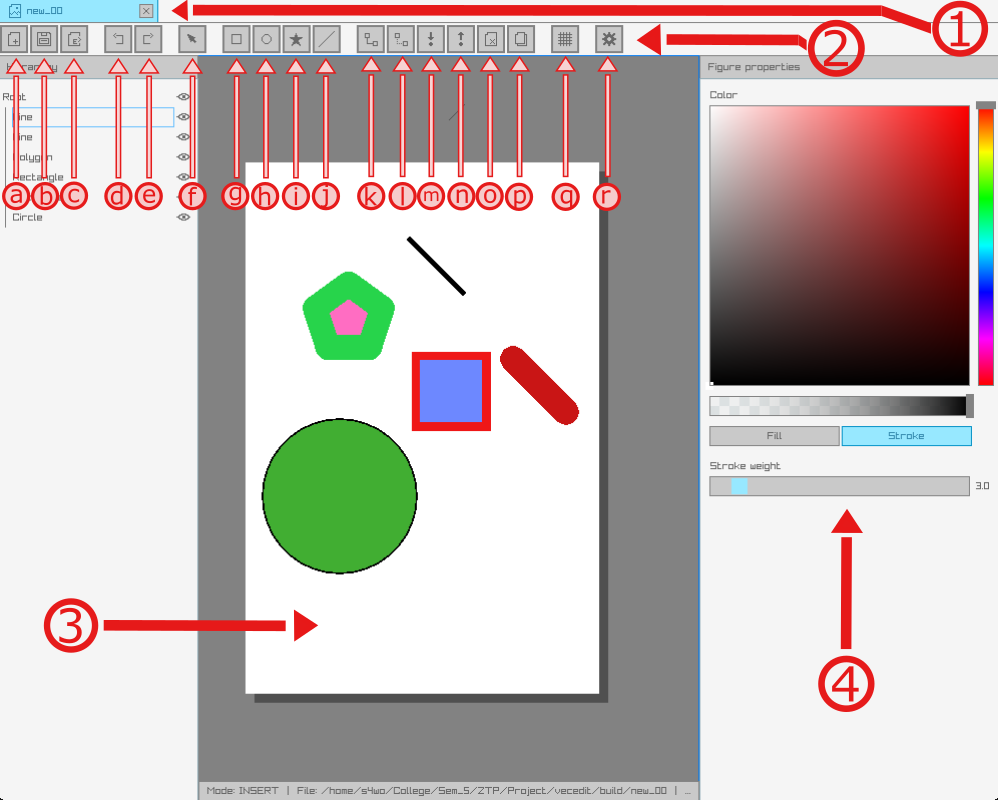
\includegraphics[width=0.75\textwidth]{./vecedit_screenshot.png}
    \caption{Przykładowy widok programu.}
    \label{fig:screenshot}
\end{figure}

\textbf{TODO: dodać opisy poszczególnych guzików}

\noindent Oznaczenia na zrzucie:
\begin{enumerate}
    \item \textbf{Pasek zakładek dokumentów} — wybór otwartego projektu, 
    możliwość zamknięcia karty.
    \item \textbf{Pasek narzędzi}:
    \begin{itemize}
      \item ikony nowego, zapisu, eksportu,
      \item przyciski \texttt{undo} i \texttt{redo},
      \item przyciski wyboru narzędzia (zaznaczanie, prostokąt, koło itp.),
      \item ikony grupowania / rozgrupowywania.
    \end{itemize}
    \item \textbf{Obszar roboczy} — kliknięcie w tym obszarze wstawia figurę 
    (jeśli wybrano narzędzie \emph{Insert}), zaznacza figurę (jeśli wybrano 
    narzędzie \emph{Select}) itp.
    \item \textbf{Panel właściwości} (z boku lub w oknie) — służy do zmiany 
    kolorów, grubości obrysu itd. dla wybranej figury.
\end{enumerate}

\subsection{Podstawowe operacje}

\textbf{TODO: usunąć/zmienić żeby było dla wszystkich guzików (razem ze skrótami klawiszowymi)}

\begin{itemize}
    \item \textbf{Nowy dokument:} \texttt{Ctrl+N} lub ikona \emph{New}.
    \item \textbf{Zapisz:} \texttt{Ctrl+S} lub ikona \emph{Save}.
    \item \textbf{Eksport do PNG:} \texttt{Ctrl+E} lub ikona \emph{Export}.
    \item \textbf{Cofnij/Ponów:} \texttt{Ctrl+Z} / \texttt{Ctrl+Y}.
    \item \textbf{Grupowanie i rozgrupowywanie:} \texttt{Ctrl+G} i \texttt{Ctrl+U}.
    \item \textbf{Klonowanie figury:} zaznacz figurę, wciśnij \texttt{Ctrl+D} 
    — powstanie duplikat w tym samym miejscu.
\end{itemize}

\section{Instrukcja instalacji i kompilacji}
\begin{enumerate}
    \item \textbf{Pobranie kodu:} Sklonuj repozytorium (np. \texttt{git clone <URL>}).
    \item \textbf{Kompilacja z użyciem CMake} (proces dokładnie opisany w \texttt{README.md}):
    \item \textbf{TODO - kompilacja w CLion}
\begin{verbatim}
mkdir build
cd build
cmake ..
make
\end{verbatim}
    \item \textbf{Raylib 5.5}: CMake spróbuje automatycznie pobrać i
      skompilować odpowiednią wersję biblioteki.
    \item \textbf{Uruchomienie}: Po kompilacji w folderze \texttt{build} znajduje się 
    plik \texttt{VecEdit} (Linux/macOS) lub \texttt{VecEdit.exe} (Windows). 
    Można go uruchomić z wiersza poleceń lub przez dwuklik. 
    \item \textbf{Problemy w macOS:} Niekiedy wymagane jest potwierdzenie
    w oknie ostrzeżeń systemu (niepodpisana aplikacja).
\end{enumerate}

\section{Podział pracy w zespole}

\section{Podsumowanie}
\texttt{VecEdit} stanowi przykład aplikacji, w~której zastosowanie wielu wzorców
projektowych (kompozyt, metoda wytwórcza, strategia, adapter, odwiedzający,
prototyp i command) umożliwia elastyczną i czytelną strukturę kodu:
\begin{itemize}
    \item \textbf{Composite} — wspólna obsługa figur i grup (hierarchii),
    \item \textbf{Factory Method} — tworzenie edytorów punktów figur,
    \item \textbf{Strategy} — łatwe definiowanie akcji dla GUI,
    \item \textbf{Adapter} — jednolite API do edycji różnych typów figur,
    \item \textbf{Visitor} — rozdzielenie logiki rysowania i serializacji,
    \item \textbf{Prototype} — proste klonowanie figur,
    \item \textbf{Command} — mechanizm cofania i ponawiania operacji.
\end{itemize}

Dzięki temu kod można łatwo rozwijać (dodawać nowe rodzaje figur, strategie, odwiedzających) 
i utrzymywać.

\vspace{1em}
\noindent
\textbf{Miłego korzystania z \texttt{VecEdit}!}

\end{document}

